% Provisional manuscript: completed results from Phases 2 and 3 only.
% Phase 4 will be inserted before Discussion; do not infer missing results.
\documentclass[aps,pra,reprint,floatfix,amsmath,amssymb,groupedaddress]{revtex4-2}
\usepackage{graphicx}
\usepackage{float}
\usepackage{bm}
\usepackage{hyperref}
\hypersetup{hidelinks}
\graphicspath{{figuras/}}

\begin{document}

\title{Exchange cycles of few ideal bosons in a one-dimensional trap: exact benchmarks for path-integral Monte Carlo}
\author{Camilo Guzm\'an}
\author{Santiago Sabogal}
\author{Milena Barrios}
\affiliation{Universidad Nacional de Colombia, Bogot\'a, Colombia}
\date{\today}

\begin{abstract}
We benchmark path-integral Monte Carlo (PIMC) with permuted endpoints for two to four noninteracting spinless bosons in a one-dimensional harmonic trap. Exact canonical partition functions derived from permutation cycles are checked independently in the occupation-number basis. The sampled full-cycle probabilities increase on cooling and approach the finite-$N$ limits $1/N$. Reconstructed partition functions and energies agree with the exact controls within the reported statistical uncertainties. With the exact Mehler kernel, changing the number of imaginary-time slices introduces no Trotter error; a separate slice study checks the sampling implementation. This finite-system benchmark establishes a controlled starting point for a change of external confinement.
\end{abstract}

\maketitle

\section{Introduction}

For identical bosons, the thermal trace includes exchanges of particle labels. In a path integral these appear as worldlines whose endpoints close under a permutation, whereas a calculation that retains only labeled periodic paths samples the identity sector. Exchange cycles therefore provide a direct, finite-system measure of the statistical contribution to the partition function \cite{feynman1948,feynman1953,ceperley1995}. The present study uses $N=2$ as an analytic control and extends the same sampler to $N=3,4$. The goal is to establish both the canonical normalization and the equilibrium frequencies of cycle classes before changing the confinement. No thermodynamic phase transition is inferred from these few-particle calculations.

\section{Theory and numerical method}

\subsection{Canonical trace and cycle weights}

We consider $N$ spinless ideal bosons in one dimension, with $H_N=\sum_{i=1}^{N}[p_i^2/(2m)+m\omega^2x_i^2/2]$. For $\beta=(k_{\mathrm B}T)^{-1}$, bosonic symmetrization gives
\begin{equation}
Z_N^{\mathrm B}=\frac{1}{N!}\sum_{\sigma\in S_N}\int dR\,
\langle R|e^{-\beta H_N}|\sigma R\rangle .
\label{eq:trace}
\end{equation}
An $\ell$-cycle joins $\ell$ one-particle propagators into a trace at inverse temperature $\ell\beta$. Writing $z_\ell\equiv z(\ell\beta)$, where
\begin{equation}
z(b)=\mathrm{Tr}\,e^{-bH_1}
=\left[2\sinh\!\left(\frac{b\hbar\omega}{2}\right)\right]^{-1},
\label{eq:z1}
\end{equation}
a class $\lambda=(1^{n_1}2^{n_2}\cdots)$ has $\sum_\ell\ell n_\ell=N$, multiplicity $g_\lambda=N!/\prod_\ell(\ell^{n_\ell}n_\ell!)$, and probability
\begin{equation}
p_\lambda=\frac{g_\lambda}{N!Z_N^{\mathrm B}}
\prod_\ell z_\ell^{n_\ell}.
\label{eq:class}
\end{equation}
In particular, $Z_2^{\mathrm B}=(z_1^2+z_2)/2$ and the exchange probability is
\begin{equation}
p_{(2)}=\frac{z_2}{z_1^2+z_2}
=\frac{1-e^{-\beta\hbar\omega}}{2}.
\label{eq:exchange2}
\end{equation}
The occupation-number basis provides an independent normalization control:
\begin{equation}
Z_N^{\mathrm{occ}}=
\frac{e^{-N\beta\hbar\omega/2}}
{\prod_{j=1}^{N}(1-e^{-j\beta\hbar\omega})}.
\label{eq:occupation}
\end{equation}
The exact energy follows from $E_N=-\partial_\beta\ln Z_N^{\mathrm{occ}}$. Equations~(\ref{eq:class}) and (\ref{eq:occupation}) agree to machine precision in the parameter grid described below.

\subsection{Permuted-endpoint PIMC}

A configuration consists of bead positions $x_{i,k}$ ($i=1,\ldots,N$, $k=0,\ldots,P-1$) and a permutation $\sigma$, with closure $x_{i,P}=x_{\sigma(i),0}$ and $\tau=\beta/P$. Its weight is
\begin{equation}
W(\bm{x},\sigma)=\prod_{i=1}^{N}\prod_{k=0}^{P-1}
\rho_1(x_{i,k},x_{i,k+1};\tau),
\label{eq:weight}
\end{equation}
where $\rho_1$ is the exact Mehler density matrix of the harmonic oscillator. Each sweep conditionally refreshes bead positions, proposes collective cycle moves, and attempts a transposition of two permutation images. For $N=3,4$, a Gaussian draw of a complete cycle is also available because Eq.~(\ref{eq:weight}) is quadratic. The transposition is accepted with $\min(1,W_{\rm new}/W_{\rm old})$; only its closure links enter this ratio. The measured exchange frequency is the equilibrium fraction of configurations in a sector, not the acceptance rate of transpositions.

The simulations use $\hbar=m=k_{\mathrm B}=\omega=1$ and $P=4$ unless stated otherwise. The $N=2$ control contains three independent chains with $8000$ measurements per temperature; $N=3,4$ use three chains with $4000$ measurements and $500$ discarded sweeps. The diagnostic repeat at $N=3$, $\beta=1$ uses $12000$ measurements and $2000$ discarded sweeps per chain. The initial seven-temperature $N=3,4$ scan used conservative block and between-chain errors; the closure runs additionally estimate integrated autocorrelations. A cycle class in the closure scan is called resolved only if it is visited at least $20$ times and has at least $100$ effective samples in every chain. The absolute partition function is reconstructed from the identity probability as
\begin{equation}
\widehat Z_N=\frac{z_1^N}{N!\,\widehat p_{(1^N)}}.
\label{eq:reconstruct}
\end{equation}
The factor $1/N!$ is inserted analytically in Eq.~(\ref{eq:reconstruct}); its independent check comes from Eq.~(\ref{eq:occupation}), not from the reconstruction alone.

\section{Results in harmonic confinement}

Figure~\ref{fig:exchange} compares full-cycle probabilities with the canonical expressions. At $\beta\hbar\omega=10$, $p_{(2)}^{\rm MC}=0.50008\pm0.00094$, versus $0.49998$ exactly. The longer $N=3$, $\beta\hbar\omega=1$ repeat gives $p_{(3)}^{\rm MC}=0.17894\pm0.00540$, versus $0.18219$. For $N=4$ at $\beta\hbar\omega=10$, $p_{(4)}^{\rm MC}=0.24842\pm0.00486$, versus $0.24999$. The limits are $p_{(N)}\to0$ at high temperature and $p_{(N)}\to1/N$ at low temperature. The rare full cycles at $\beta\hbar\omega=0.1$ for $N=3,4$ do not meet the preset resolution threshold and are omitted as Monte Carlo points; the exact curves extend to that limit.

\begin{figure}[t]
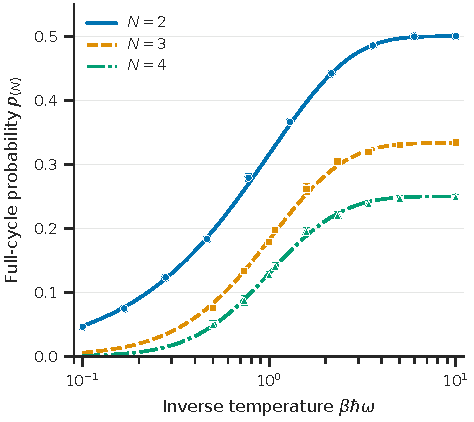
\includegraphics[width=\columnwidth]{exchange_cycles.pdf}
\caption{Full-cycle probability for $N=2,3,4$ versus inverse temperature. Curves are exact canonical results; symbols are independent-chain PIMC estimates with one-standard-error bars. The $N=3$, $\beta\hbar\omega=1$ symbol uses the longer diagnostic repeat. Unresolved high-temperature full-cycle estimates for $N=3,4$ are omitted.}
\label{fig:exchange}
\end{figure}

The cycle and occupation formulas were compared for $N=2,3,4$, seven temperatures, and three trap frequencies: the largest relative partition-function discrepancy among the $63$ controls was $2.1\times10^{-15}$. Figure~\ref{fig:partition} checks the separate PIMC reconstruction. For $N=4$, the ratio $\widehat Z_4/Z_4^{\mathrm{occ}}$ ranges from $0.969$ to $1.004$ across $\beta\hbar\omega=0.1,1,10$ and remains compatible with unity within the estimated errors. At $\beta\hbar\omega=10$, the thermodynamic energy is $E_4^{\rm MC}=2.00084\pm0.00091$, versus $E_4^{\rm exact}=2.00005$.

Figure~\ref{fig:energy} traces the thermodynamic energy across the same temperature range. It approaches the classical high-temperature scale $N/\beta$ and the $N\hbar\omega/2$ ground-state limit without evidence of a systematic deviation from the occupation-basis curve. This energy control probes the sampled coordinate distribution in addition to the permutation-sector frequencies.

Figure~\ref{fig:classes4} resolves the five distinct cycle classes of $S_4$. At $\beta\hbar\omega=1$, the measured probabilities of the identity, $1+1+2$, $1+3$, $2+2$, and $4$ classes are $0.1326$, $0.3683$, $0.2882$, $0.0841$, and $0.1269$, respectively; the exact values are $0.1331$, $0.3689$, $0.2829$, $0.0852$, and $0.1298$. At low temperature, these probabilities tend to the multiplicity ratios $1:6:8:3:6$ divided by $24$. The full class structure is therefore more informative than a binary ``exchange/no exchange'' count.

The explicit $P$ scan in Fig.~\ref{fig:pcheck} includes $N=3,4$ at $\beta\hbar\omega=0.5,1,5$. Across these $24$ settings, the largest resolved-class residual from the exact probability was $2.55$ estimated standard errors; the largest pairwise difference between two $P$ values of the same class was $2.79$ combined errors. No systematic drift is visible. The exact Mehler kernel makes this a sampling check rather than a Trotter extrapolation. At $P=4$ and $\beta\hbar\omega=1$, the whole-cycle Gaussian update yields $297$ versus $205$ effective energy samples per second for $N=3$, and $398$ versus $131$ for $N=4$, compared with the local-only variant. These timings are implementation and hardware dependent; their detailed comparison is in the Supplemental Material.

\begin{figure}[t]
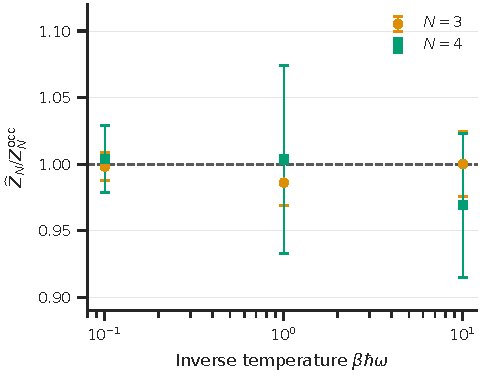
\includegraphics[width=\columnwidth]{partition_check.pdf}
\caption{Partition functions reconstructed through Eq.~(\ref{eq:reconstruct}) and divided by the independent occupation-basis result, Eq.~(\ref{eq:occupation}). Error bars propagate the uncertainty of the sampled identity-sector probability. The dashed line denotes exact agreement.}
\label{fig:partition}
\end{figure}

\begin{figure*}[t]
\centering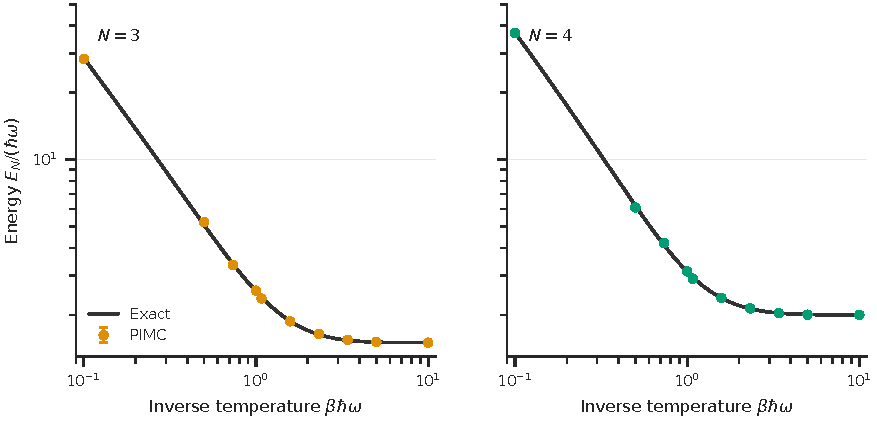
\includegraphics[width=.94\textwidth]{energy_control.pdf}
\caption{Thermodynamic energy for $N=3$ and $N=4$ across the harmonic-trap temperature scan. Solid curves follow the independent occupation-basis expression $E_N=-\partial_\beta\ln Z_N^{\rm occ}$; symbols are PIMC means with one-standard-error bars. The ordinate is logarithmic to display both the classical and ground-state regimes.}
\label{fig:energy}
\end{figure*}

\begin{figure}[t]
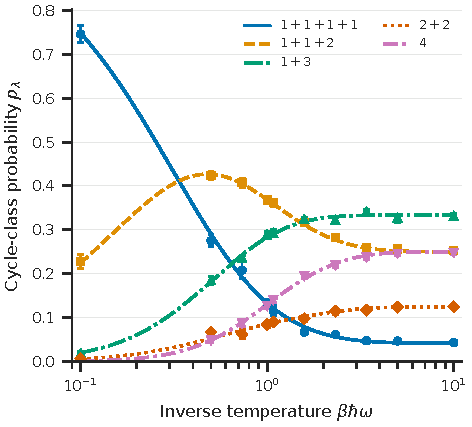
\includegraphics[width=\columnwidth]{class_probabilities_N4.pdf}
\caption{Probabilities of the five permutation-cycle classes for four bosons. Curves are exact canonical weights and symbols are PIMC estimates with one-standard-error bars. The unresolved full-cycle point at $\beta\hbar\omega=0.1$ is omitted. The ordering and limiting values reflect the class multiplicities in $S_4$.}
\label{fig:classes4}
\end{figure}

\begin{figure*}[t]
\centering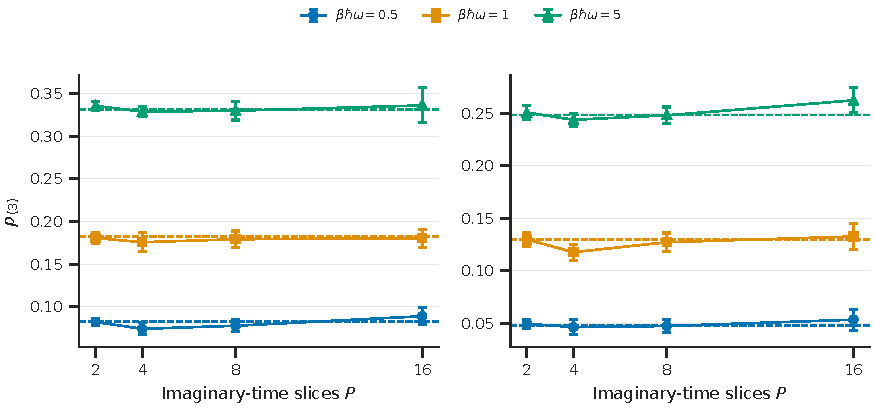
\includegraphics[width=.94\textwidth]{p_convergence.pdf}
\caption{Full-cycle probabilities for $N=3$ (left) and $N=4$ (right) across $P=2,4,8,16$ at three temperatures. Horizontal dashed lines are exact canonical values; symbols are three-chain PIMC estimates with one-standard-error bars. Color and marker shape identify inverse temperature. The absence of a systematic trend is expected for the exact harmonic propagator.}
\label{fig:pcheck}
\end{figure*}

% PHASE 4 INSERTION POINT: add the new external potential, propagator,
% independent one-body spectral control, convergence in P, and comparison
% figures here. Revise the abstract, title, discussion, and conclusions.

\section{Discussion}

The two thermal limits follow directly from the cycle weights. For $\beta\hbar\omega\ll1$, $z(\ell\beta)\simeq(\ell\beta\hbar\omega)^{-1}$, so a class with $C=\sum_\ell n_\ell$ cycles has weight proportional to $\beta^{-C}$. The identity class has the largest $C=N$ and dominates. For $\beta\hbar\omega\gg1$, every permutation has the same leading ground-state factor $e^{-N\beta\hbar\omega/2}$, leaving only the class multiplicities. Thus the increasing exchange frequencies are a continuous finite-$N$ crossover fixed by the spectrum and permutation counting.

The agreement tests have different logical roles. The occupation-basis formula is independent of the permutation enumeration and checks the global $1/N!$ normalization. By contrast, $\widehat Z_N$ is calculated from the same identity-sector frequency used in the class histogram; those two Monte Carlo checks are correlated. The energy estimator uses the same sampled paths, so its agreement adds an observable check but does not provide another independent Monte Carlo chain.

A rising full-cycle probability characterizes exchange within the finite canonical system, without establishing condensation. Sampling diagnostics matter even when ensemble means agree with exact values: one short $N=3$, $\beta\hbar\omega=1$ chain showed a $3.67$-standard-error difference between its halves after autocorrelation correction. The longer independent repeat reduced the largest corresponding discrepancy to $1.69$ errors. The complete-cycle Gaussian update increased effective energy samples per second in the tested $P=4$, $\beta\hbar\omega=1$ cases, but its exact form relies on the harmonic action.

% Draft layout break: remove when the Phase 4 section is inserted above.
\newpage
Changing an external one-body potential changes $z(\beta)$ and hence the temperature dependence in Eq.~(\ref{eq:class}), while the permutation multiplicities and the bosonic $1/N!$ factor remain fixed. A nonharmonic calculation will also require separating finite-$P$ bias from Monte Carlo uncertainty. These distinctions define the controlled comparison to be made in the confinement extension.

\section{Conclusions}

Permuted-endpoint PIMC reproduces the canonical exchange-cycle frequencies and thermal observables of two to four ideal trapped bosons. The occupation-basis calculation independently verifies the symmetrization normalization. These controls establish the reference against which a different external confinement can be evaluated; that extension has not yet been simulated and is excluded from the present numerical claims.

\section*{Data and code availability}

The simulation code, input parameters, saved Monte Carlo series, numerical summaries underlying every figure, and figure-generation scripts are available in the versioned repository \cite{bosones_code_v1}. The repository documents the dependencies and commands used to reproduce the results.

\bibliographystyle{apsrev4-2}
\bibliography{references}

% The six-page limit applies to the main text above. The following
% illustrated appendices are in this same PDF, after the bibliography.
\clearpage
\onecolumngrid
\appendix

\section{Worldline closure and two-boson controls}

Figure~\ref{fig:app-topology} depicts the endpoint condition in Eq.~(\ref{eq:trace}). It is a schematic of the two topological sectors, not a measured trajectory. Figures~\ref{fig:app-two-control} and \ref{fig:app-two-energy} retain the separate $N=2$ checks that were combined or summarized in the main text. Their Monte Carlo points come from the same $P=4$ temperature sweep, with three chains of 8000 measurements per temperature; agreement among these derived observables must not be counted as independent statistical evidence.

\begin{figure}[H]
\centering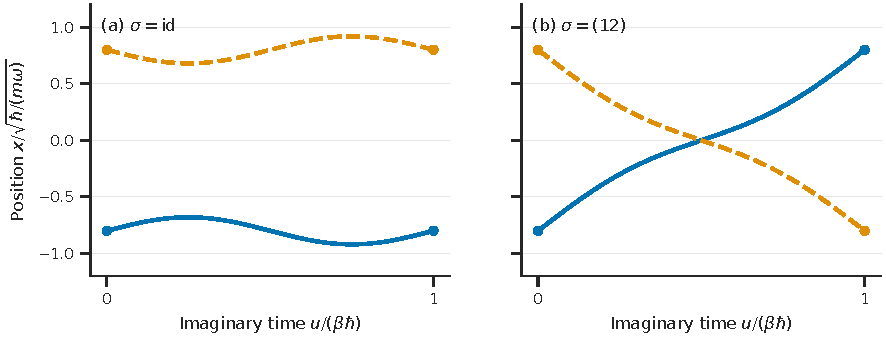
\includegraphics[width=.84\textwidth]{worldline_topology.pdf}
\caption{Schematic closure of two worldlines in imaginary time. (a) The identity permutation closes each path on its own starting point, producing two cycles of length $\beta\hbar$. (b) The transposition joins the two paths into one cycle of length $2\beta\hbar$: $x_i(\beta\hbar)=x_{\sigma(i)}(0)$. Curves illustrate topology only; they are not sampled positions.}
\label{fig:app-topology}
\end{figure}

\begin{figure}[H]
\centering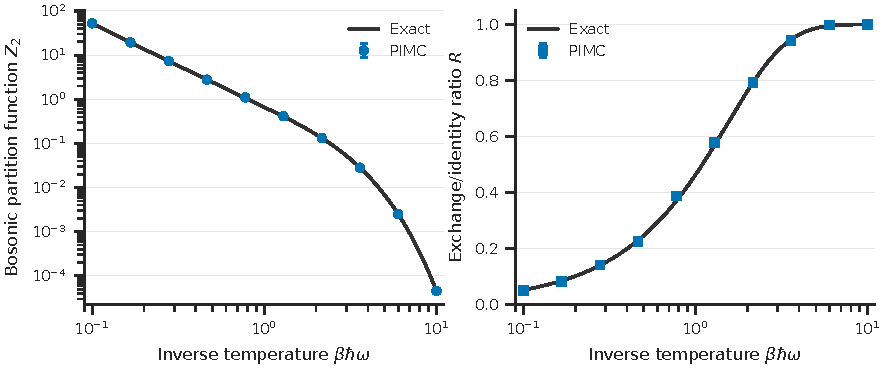
\includegraphics[width=.91\textwidth]{phase2_partition_ratio.pdf}
\caption{Two-boson normalization and exchange-sector controls. Left: $Z_2^{\rm B}=(z_1^2+z_2)/2$ (line) versus $\widehat Z_2=z_1^2/[2(1-\widehat p_{(2)})]$ (points). Right: the exchange-to-identity weight ratio $R=z_2/z_1^2=\tanh(\beta\hbar\omega/2)$ versus $\widehat R=\widehat p_{(2)}/(1-\widehat p_{(2)})$. One-standard-error bars are propagated from the same measured exchange fraction; the panels are therefore correlated.}
\label{fig:app-two-control}
\end{figure}

\begin{figure}[H]
\centering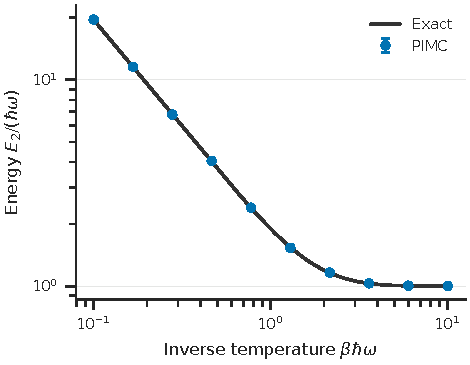
\includegraphics[width=.55\textwidth]{phase2_energy.pdf}
\caption{Thermodynamic energy of two bosons. The line is $E_2=-\partial_\beta\ln Z_2^{\rm B}$ from the exact partition function, and points are PIMC estimates from the derivative of the Mehler-link weight. Error bars combine within-chain block estimates and between-chain spread. The low-temperature limit is $\hbar\omega$; the high-temperature leading term is $2/\beta$.}
\label{fig:app-two-energy}
\end{figure}

\section{Full class and particle-cycle distributions}

For $N=3$, Fig.~\ref{fig:app-three-classes} retains all permutation classes. Figure~\ref{fig:app-histograms} shows a common-temperature snapshot for $N=3$ and $N=4$, while Fig.~\ref{fig:app-particle-fractions} counts particles rather than configurations. These plots are different projections of the same sampled permutations; their statistical errors and deviations from the exact curves are correlated.

\begin{figure}[H]
\centering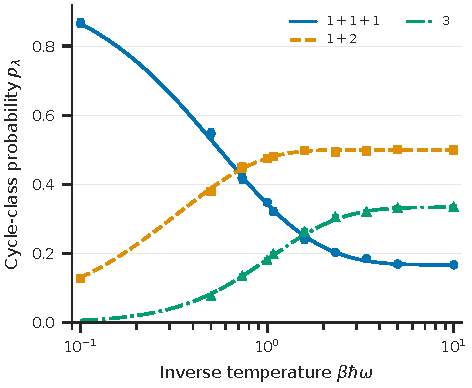
\includegraphics[width=.58\textwidth]{class_probabilities_N3.pdf}
\caption{Three-boson probabilities for classes $1+1+1$, $1+2$, and $3$. Curves are the canonical values from Eq.~(\ref{eq:class}); symbols are PIMC means with one-standard-error bars. The $\beta\hbar\omega=1$ point uses the longer repeat. The rare full-cycle point at $\beta\hbar\omega=0.1$ fails the prespecified count threshold and is omitted, although its exact curve is shown.}
\label{fig:app-three-classes}
\end{figure}

\begin{figure}[H]
\centering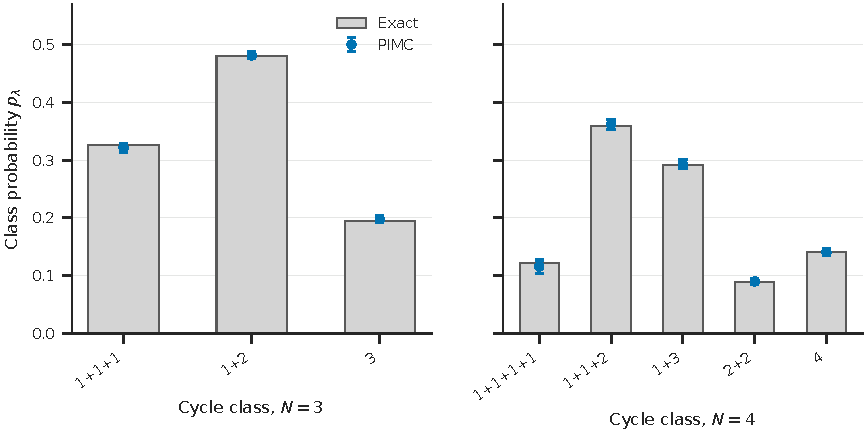
\includegraphics[width=.91\textwidth]{class_histograms.pdf}
\caption{Class-by-class snapshot at $\beta\hbar\omega=1.077$ for $N=3$ (left) and $N=4$ (right). Gray bars are exact canonical probabilities; colored points and one-standard-error bars come from three independent PIMC chains with 4000 measurements each. Errors here use block and between-chain estimates from the historical sweep. The separate classes $1+1+2$ and $2+2$ have different multiplicities despite both containing a two-cycle.}
\label{fig:app-histograms}
\end{figure}

\begin{figure}[H]
\centering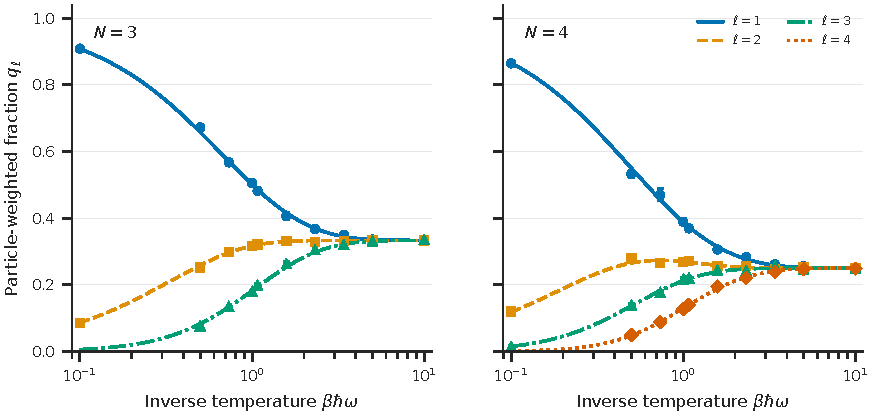
\includegraphics[width=.91\textwidth]{particle_cycle_fractions.pdf}
\caption{Particle-weighted cycle fractions $q_\ell=\ell\langle n_\ell\rangle/N$ for $N=3$ (left) and $N=4$ (right), with $\sum_\ell q_\ell=1$. Curves follow the exact class weights; symbols are PIMC means and one-standard-error bars. Unlike $p_\lambda$, $q_\ell$ is the probability that a randomly chosen particle belongs to a cycle of length $\ell$. Points that depend on unresolved rare classes at $\beta\hbar\omega=0.1$ are omitted. Each $q_\ell\to1/N$ as $\beta\hbar\omega\to\infty$.}
\label{fig:app-particle-fractions}
\end{figure}

\clearpage
\section{Sampling-cost diagnostic}

Figure~\ref{fig:app-cost} documents the cost of exploring permutation sectors. The acceptance rate of transpositions is not itself an estimate of an equilibrium class probability, and a shorter integrated autocorrelation time does not necessarily imply lower wall-clock cost. The plotted effective-sample rate combines both effects but has no independently estimated timing confidence interval.

\begin{figure}[H]
\centering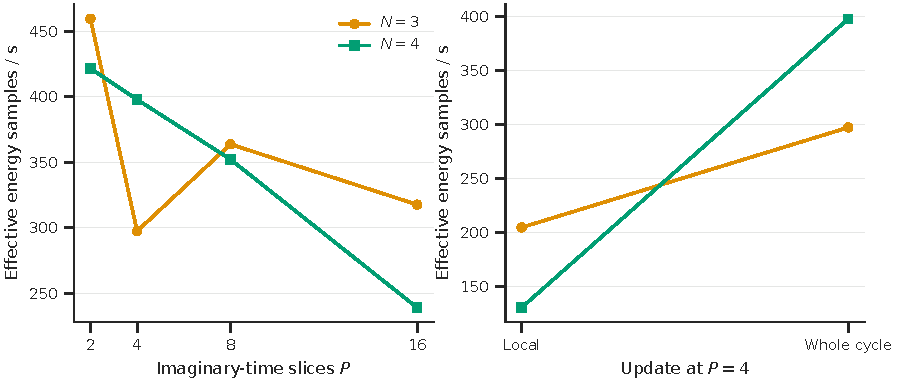
\includegraphics[width=.91\textwidth]{sampling_cost.pdf}
\caption{Effective energy samples per second at $\beta\hbar\omega=1$. Left: dependence on the number of slices $P$ with complete-cycle Gaussian refresh. Right: local-only and complete-cycle updates at $P=4$. Each setting has three replicas with the same seed base and 500 discarded sweeps; complete-cycle runs use 2500 measurements per replica, while local-only runs use 4000. These values describe this implementation and computer. The unequal run lengths and absence of timing error bars make the apparent speedups descriptive rather than a controlled universal performance estimate.}
\label{fig:app-cost}
\end{figure}

\end{document}
